% Options for packages loaded elsewhere
\PassOptionsToPackage{unicode}{hyperref}
\PassOptionsToPackage{hyphens}{url}
%
\documentclass[
]{article}
\usepackage{amsmath,amssymb}
\usepackage{iftex}
\ifPDFTeX
  \usepackage[T1]{fontenc}
  \usepackage[utf8]{inputenc}
  \usepackage{textcomp} % provide euro and other symbols
\else % if luatex or xetex
  \usepackage{unicode-math} % this also loads fontspec
  \defaultfontfeatures{Scale=MatchLowercase}
  \defaultfontfeatures[\rmfamily]{Ligatures=TeX,Scale=1}
\fi
\usepackage{lmodern}
\ifPDFTeX\else
  % xetex/luatex font selection
\fi
% Use upquote if available, for straight quotes in verbatim environments
\IfFileExists{upquote.sty}{\usepackage{upquote}}{}
\IfFileExists{microtype.sty}{% use microtype if available
  \usepackage[]{microtype}
  \UseMicrotypeSet[protrusion]{basicmath} % disable protrusion for tt fonts
}{}
\makeatletter
\@ifundefined{KOMAClassName}{% if non-KOMA class
  \IfFileExists{parskip.sty}{%
    \usepackage{parskip}
  }{% else
    \setlength{\parindent}{0pt}
    \setlength{\parskip}{6pt plus 2pt minus 1pt}}
}{% if KOMA class
  \KOMAoptions{parskip=half}}
\makeatother
\usepackage{xcolor}
\usepackage[margin=1in]{geometry}
\usepackage{color}
\usepackage{fancyvrb}
\newcommand{\VerbBar}{|}
\newcommand{\VERB}{\Verb[commandchars=\\\{\}]}
\DefineVerbatimEnvironment{Highlighting}{Verbatim}{commandchars=\\\{\}}
% Add ',fontsize=\small' for more characters per line
\usepackage{framed}
\definecolor{shadecolor}{RGB}{248,248,248}
\newenvironment{Shaded}{\begin{snugshade}}{\end{snugshade}}
\newcommand{\AlertTok}[1]{\textcolor[rgb]{0.94,0.16,0.16}{#1}}
\newcommand{\AnnotationTok}[1]{\textcolor[rgb]{0.56,0.35,0.01}{\textbf{\textit{#1}}}}
\newcommand{\AttributeTok}[1]{\textcolor[rgb]{0.13,0.29,0.53}{#1}}
\newcommand{\BaseNTok}[1]{\textcolor[rgb]{0.00,0.00,0.81}{#1}}
\newcommand{\BuiltInTok}[1]{#1}
\newcommand{\CharTok}[1]{\textcolor[rgb]{0.31,0.60,0.02}{#1}}
\newcommand{\CommentTok}[1]{\textcolor[rgb]{0.56,0.35,0.01}{\textit{#1}}}
\newcommand{\CommentVarTok}[1]{\textcolor[rgb]{0.56,0.35,0.01}{\textbf{\textit{#1}}}}
\newcommand{\ConstantTok}[1]{\textcolor[rgb]{0.56,0.35,0.01}{#1}}
\newcommand{\ControlFlowTok}[1]{\textcolor[rgb]{0.13,0.29,0.53}{\textbf{#1}}}
\newcommand{\DataTypeTok}[1]{\textcolor[rgb]{0.13,0.29,0.53}{#1}}
\newcommand{\DecValTok}[1]{\textcolor[rgb]{0.00,0.00,0.81}{#1}}
\newcommand{\DocumentationTok}[1]{\textcolor[rgb]{0.56,0.35,0.01}{\textbf{\textit{#1}}}}
\newcommand{\ErrorTok}[1]{\textcolor[rgb]{0.64,0.00,0.00}{\textbf{#1}}}
\newcommand{\ExtensionTok}[1]{#1}
\newcommand{\FloatTok}[1]{\textcolor[rgb]{0.00,0.00,0.81}{#1}}
\newcommand{\FunctionTok}[1]{\textcolor[rgb]{0.13,0.29,0.53}{\textbf{#1}}}
\newcommand{\ImportTok}[1]{#1}
\newcommand{\InformationTok}[1]{\textcolor[rgb]{0.56,0.35,0.01}{\textbf{\textit{#1}}}}
\newcommand{\KeywordTok}[1]{\textcolor[rgb]{0.13,0.29,0.53}{\textbf{#1}}}
\newcommand{\NormalTok}[1]{#1}
\newcommand{\OperatorTok}[1]{\textcolor[rgb]{0.81,0.36,0.00}{\textbf{#1}}}
\newcommand{\OtherTok}[1]{\textcolor[rgb]{0.56,0.35,0.01}{#1}}
\newcommand{\PreprocessorTok}[1]{\textcolor[rgb]{0.56,0.35,0.01}{\textit{#1}}}
\newcommand{\RegionMarkerTok}[1]{#1}
\newcommand{\SpecialCharTok}[1]{\textcolor[rgb]{0.81,0.36,0.00}{\textbf{#1}}}
\newcommand{\SpecialStringTok}[1]{\textcolor[rgb]{0.31,0.60,0.02}{#1}}
\newcommand{\StringTok}[1]{\textcolor[rgb]{0.31,0.60,0.02}{#1}}
\newcommand{\VariableTok}[1]{\textcolor[rgb]{0.00,0.00,0.00}{#1}}
\newcommand{\VerbatimStringTok}[1]{\textcolor[rgb]{0.31,0.60,0.02}{#1}}
\newcommand{\WarningTok}[1]{\textcolor[rgb]{0.56,0.35,0.01}{\textbf{\textit{#1}}}}
\usepackage{longtable,booktabs,array}
\usepackage{calc} % for calculating minipage widths
% Correct order of tables after \paragraph or \subparagraph
\usepackage{etoolbox}
\makeatletter
\patchcmd\longtable{\par}{\if@noskipsec\mbox{}\fi\par}{}{}
\makeatother
% Allow footnotes in longtable head/foot
\IfFileExists{footnotehyper.sty}{\usepackage{footnotehyper}}{\usepackage{footnote}}
\makesavenoteenv{longtable}
\usepackage{graphicx}
\makeatletter
\def\maxwidth{\ifdim\Gin@nat@width>\linewidth\linewidth\else\Gin@nat@width\fi}
\def\maxheight{\ifdim\Gin@nat@height>\textheight\textheight\else\Gin@nat@height\fi}
\makeatother
% Scale images if necessary, so that they will not overflow the page
% margins by default, and it is still possible to overwrite the defaults
% using explicit options in \includegraphics[width, height, ...]{}
\setkeys{Gin}{width=\maxwidth,height=\maxheight,keepaspectratio}
% Set default figure placement to htbp
\makeatletter
\def\fps@figure{htbp}
\makeatother
\setlength{\emergencystretch}{3em} % prevent overfull lines
\providecommand{\tightlist}{%
  \setlength{\itemsep}{0pt}\setlength{\parskip}{0pt}}
\setcounter{secnumdepth}{-\maxdimen} % remove section numbering
\ifLuaTeX
  \usepackage{selnolig}  % disable illegal ligatures
\fi
\IfFileExists{bookmark.sty}{\usepackage{bookmark}}{\usepackage{hyperref}}
\IfFileExists{xurl.sty}{\usepackage{xurl}}{} % add URL line breaks if available
\urlstyle{same}
\hypersetup{
  pdftitle={Bayes},
  pdfauthor={Aldona Swirad},
  hidelinks,
  pdfcreator={LaTeX via pandoc}}

\title{Bayes}
\author{Aldona Swirad}
\date{}

\begin{document}
\maketitle

\section{Dane}\label{dane}

Zestaw danych zawiera 18 zmiennych (9 wartości logicznych, 5 ciągów
znaków i 4 liczby dziesiętne). W projektach związanych z uczeniem
maszynowym ``HeartDisease'' może być wykorzystywane jako zmienna
objaśniająca, ale należy zauważyć, że klasy są silnie niezrównoważone.

Dane pobrane zostały z kaggle:
\url{https://www.kaggle.com/code/georgyzubkov/heart-disease-exploratory-data-analysis/input}.
Dane zawierają takie cechy jak:

\section{Opis cech:}\label{opis-cech}

\begin{itemize}
\item
  \textbf{HeartDisease} - czy badany ma chorobę serca.
\item
  \textbf{BMI} - wartość, która pozwala ocenić stopień zgodności masy
  ciała osoby z jej wzrostem, a tym samym pośrednio ocenić, czy masa
  jest niewystarczająca, normalna czy nadmierna. Jest to ważne przy
  ustalaniu wskazań do konieczności leczenia.
\item
  \textbf{Smoking} - palenie jest głównym czynnikiem ryzyka chorób
  sercowo-naczyniowych. Po inhalacji dymu z papierosa reakcja układu
  sercowo-naczyniowego następuje natychmiastowo: w ciągu jednej minuty
  tempo akcji serca zaczyna wzrastać, zwiększając się o 30\% w ciągu
  dziesięciu minut palenia. Zły nawyk również podnosi ciśnienie krwi,
  poziom fibrinogenu i płytek krwi, co zwiększa prawdopodobieństwo
  powstawania skrzepów.
\item
  \textbf{AlcoholDrinking} - alkohol powoduje nie tylko tymczasowe
  zaburzenia w funkcjonowaniu serca, ale także trwałe. Ból serca po
  alkoholu to nie jedyny problem zdrowotny związany z jego spożyciem.
\item
  \textbf{Stroke} - Udar niedokrwienny występuje 4 razy częściej niż
  krwotoczny. Jedną z głównych przyczyn tego cierpienia są choroby
  serca, które upośledzają jego funkcjonowanie, w wyniku czego przepływ
  krwi w tętnicach jest zakłócony, a dopływ krwi do mózgu zmniejszony.
  Inną przyczyną udaru w chorobach serca jest zakrzepica, gdy powstają
  skrzepy w jamach serca (najczęściej przy niewydolności serca) -
  skrzepy krwi.
\item
  \textbf{PhysicalHealth} - ile dni w miesiącu badany czuł się zle pod
  kątem zdrowia fizycznego.
\item
  \textbf{MentalHealth} - ile dni w miesiącu badany czuł się zle pod
  kątem zdrowia psychicznego.
\item
  \textbf{DiffWalking} - trudność w wchodzeniu po schodach.
\item
  \textbf{Sex} - płeć osoby.
\item
  \textbf{AgeCategory} - kategoria wiekowa badanych.
\item
  \textbf{Race} - rasa.
\item
  \textbf{Diabetic} - cukrzyca.
\item
  \textbf{PhysicalActivity} - badano, którzy zgłosili wykonywanie
  aktywności fizycznej lub ćwiczeń w ciągu ostatnich 30 dni oprócz
  swojej regularnej pracy.
\item
  \textbf{GenHealth} - samopoczucie.
\item
  \textbf{SleepTime} - liczba godzin snu.
\item
  \textbf{Asthma} - astma.
\item
  \textbf{KidneyDisease} - choroba nerek.
\item
  \textbf{Skin Cancer} - rak skóry.
\end{itemize}

\section{Instalacja i wszystywanie potrzebnych bibliotek w środowisku
R}\label{instalacja-i-wszystywanie-potrzebnych-bibliotek-w-ux15brodowisku-r}

\begin{verbatim}
## Warning: pakiet 'readxl' został zbudowany w wersji R 4.3.3
\end{verbatim}

\begin{verbatim}
## Warning: pakiet 'bnlearn' został zbudowany w wersji R 4.3.3
\end{verbatim}

\section{Wczytywanie danych z csv}\label{wczytywanie-danych-z-csv}

\begin{longtable}[]{@{}
  >{\centering\arraybackslash}p{(\columnwidth - 12\tabcolsep) * \real{0.1647}}
  >{\centering\arraybackslash}p{(\columnwidth - 12\tabcolsep) * \real{0.0824}}
  >{\centering\arraybackslash}p{(\columnwidth - 12\tabcolsep) * \real{0.1059}}
  >{\centering\arraybackslash}p{(\columnwidth - 12\tabcolsep) * \real{0.2000}}
  >{\centering\arraybackslash}p{(\columnwidth - 12\tabcolsep) * \real{0.0941}}
  >{\centering\arraybackslash}p{(\columnwidth - 12\tabcolsep) * \real{0.1882}}
  >{\centering\arraybackslash}p{(\columnwidth - 12\tabcolsep) * \real{0.1647}}@{}}
\toprule\noalign{}
\begin{minipage}[b]{\linewidth}\centering
HeartDisease
\end{minipage} & \begin{minipage}[b]{\linewidth}\centering
BMI
\end{minipage} & \begin{minipage}[b]{\linewidth}\centering
Smoking
\end{minipage} & \begin{minipage}[b]{\linewidth}\centering
AlcoholDrinking
\end{minipage} & \begin{minipage}[b]{\linewidth}\centering
Stroke
\end{minipage} & \begin{minipage}[b]{\linewidth}\centering
PhysicalHealth
\end{minipage} & \begin{minipage}[b]{\linewidth}\centering
MentalHealth
\end{minipage} \\
\midrule\noalign{}
\endhead
\bottomrule\noalign{}
\endlastfoot
No & 16.60 & Yes & No & No & 3 & 30 \\
No & 20.34 & No & No & Yes & 0 & 0 \\
No & 26.58 & Yes & No & No & 20 & 30 \\
No & 24.21 & No & No & No & 0 & 0 \\
No & 23.71 & No & No & No & 28 & 0 \\
Yes & 28.87 & Yes & No & No & 6 & 0 \\
\end{longtable}

\begin{longtable}[]{@{}
  >{\centering\arraybackslash}p{(\columnwidth - 16\tabcolsep) * \real{0.1333}}
  >{\centering\arraybackslash}p{(\columnwidth - 16\tabcolsep) * \real{0.1238}}
  >{\centering\arraybackslash}p{(\columnwidth - 16\tabcolsep) * \real{0.0762}}
  >{\centering\arraybackslash}p{(\columnwidth - 16\tabcolsep) * \real{0.1238}}
  >{\centering\arraybackslash}p{(\columnwidth - 16\tabcolsep) * \real{0.0667}}
  >{\centering\arraybackslash}p{(\columnwidth - 16\tabcolsep) * \real{0.0952}}
  >{\centering\arraybackslash}p{(\columnwidth - 16\tabcolsep) * \real{0.1714}}
  >{\centering\arraybackslash}p{(\columnwidth - 16\tabcolsep) * \real{0.1048}}
  >{\centering\arraybackslash}p{(\columnwidth - 16\tabcolsep) * \real{0.1048}}@{}}
\toprule\noalign{}
\begin{minipage}[b]{\linewidth}\centering
MentalHealth
\end{minipage} & \begin{minipage}[b]{\linewidth}\centering
DiffWalking
\end{minipage} & \begin{minipage}[b]{\linewidth}\centering
Sex
\end{minipage} & \begin{minipage}[b]{\linewidth}\centering
AgeCategory
\end{minipage} & \begin{minipage}[b]{\linewidth}\centering
Race
\end{minipage} & \begin{minipage}[b]{\linewidth}\centering
Diabetic
\end{minipage} & \begin{minipage}[b]{\linewidth}\centering
PhysicalActivity
\end{minipage} & \begin{minipage}[b]{\linewidth}\centering
GenHealth
\end{minipage} & \begin{minipage}[b]{\linewidth}\centering
SleepTime
\end{minipage} \\
\midrule\noalign{}
\endhead
\bottomrule\noalign{}
\endlastfoot
30 & No & Female & 55-59 & White & Yes & Yes & Very good & 5 \\
0 & No & Female & 80 or older & White & No & Yes & Very good & 7 \\
30 & No & Male & 65-69 & White & Yes & Yes & Fair & 8 \\
0 & No & Female & 75-79 & White & No & No & Good & 6 \\
0 & Yes & Female & 40-44 & White & No & Yes & Very good & 8 \\
0 & Yes & Female & 75-79 & Black & No & No & Fair & 12 \\
\end{longtable}

\section{Redukcja ilości danych atrybutowych do
(5-7)}\label{redukcja-iloux15bci-danych-atrybutowych-do-5-7}

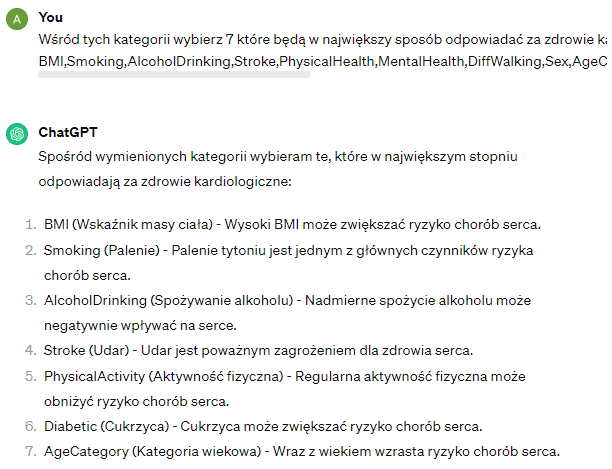
\includegraphics[width=1\linewidth]{ktore}

Pod uwage wzięłam tylko te cechy, które mają zazwyczaj największy wpły
na występowanie chorób kardiologicznych.

\begin{Shaded}
\begin{Highlighting}[]
\CommentTok{\# usuwam SkinCancer}
\NormalTok{cardio }\OtherTok{\textless{}{-}}\NormalTok{ cardio[, }\SpecialCharTok{{-}}\DecValTok{18}\NormalTok{]}
\CommentTok{\# usuwam KidneyDisease}
\NormalTok{cardio }\OtherTok{\textless{}{-}}\NormalTok{ cardio[, }\SpecialCharTok{{-}}\DecValTok{17}\NormalTok{]}
\CommentTok{\#usuwam Asthma}
\NormalTok{cardio }\OtherTok{\textless{}{-}}\NormalTok{ cardio[, }\SpecialCharTok{{-}}\DecValTok{16}\NormalTok{]}
\CommentTok{\#usuwam SleepTime}
\NormalTok{cardio }\OtherTok{\textless{}{-}}\NormalTok{ cardio[, }\SpecialCharTok{{-}}\DecValTok{15}\NormalTok{]}
\CommentTok{\#usuwam GenHealth}
\NormalTok{cardio }\OtherTok{\textless{}{-}}\NormalTok{ cardio[, }\SpecialCharTok{{-}}\DecValTok{14}\NormalTok{]}
\CommentTok{\#usuwam Race}
\NormalTok{cardio }\OtherTok{\textless{}{-}}\NormalTok{ cardio[, }\SpecialCharTok{{-}}\DecValTok{11}\NormalTok{]}
\CommentTok{\#usuwam Sex}
\NormalTok{cardio }\OtherTok{\textless{}{-}}\NormalTok{ cardio[, }\SpecialCharTok{{-}}\DecValTok{9}\NormalTok{]}
\CommentTok{\#usuwam DiffWalking}
\NormalTok{cardio }\OtherTok{\textless{}{-}}\NormalTok{ cardio[, }\SpecialCharTok{{-}}\DecValTok{8}\NormalTok{]}
\CommentTok{\#usuwam MentalHealth}
\NormalTok{cardio }\OtherTok{\textless{}{-}}\NormalTok{ cardio[, }\SpecialCharTok{{-}}\DecValTok{7}\NormalTok{]}
\CommentTok{\#usuwam PhisicalHealth}
\NormalTok{cardio }\OtherTok{\textless{}{-}}\NormalTok{ cardio[, }\SpecialCharTok{{-}}\DecValTok{6}\NormalTok{]}
\NormalTok{knitr}\SpecialCharTok{::}\FunctionTok{kable}\NormalTok{(}\FunctionTok{head}\NormalTok{(cardio), }\StringTok{"pipe"}\NormalTok{, }\AttributeTok{align =} \StringTok{"ccccc"}\NormalTok{)}
\end{Highlighting}
\end{Shaded}

\begin{longtable}[]{@{}
  >{\centering\arraybackslash}p{(\columnwidth - 14\tabcolsep) * \real{0.1458}}
  >{\centering\arraybackslash}p{(\columnwidth - 14\tabcolsep) * \real{0.0729}}
  >{\centering\arraybackslash}p{(\columnwidth - 14\tabcolsep) * \real{0.0938}}
  >{\centering\arraybackslash}p{(\columnwidth - 14\tabcolsep) * \real{0.1771}}
  >{\centering\arraybackslash}p{(\columnwidth - 14\tabcolsep) * \real{0.0833}}
  >{\centering\arraybackslash}p{(\columnwidth - 14\tabcolsep) * \real{0.1354}}
  >{\centering\arraybackslash}p{(\columnwidth - 14\tabcolsep) * \real{0.1042}}
  >{\centering\arraybackslash}p{(\columnwidth - 14\tabcolsep) * \real{0.1875}}@{}}
\toprule\noalign{}
\begin{minipage}[b]{\linewidth}\centering
HeartDisease
\end{minipage} & \begin{minipage}[b]{\linewidth}\centering
BMI
\end{minipage} & \begin{minipage}[b]{\linewidth}\centering
Smoking
\end{minipage} & \begin{minipage}[b]{\linewidth}\centering
AlcoholDrinking
\end{minipage} & \begin{minipage}[b]{\linewidth}\centering
Stroke
\end{minipage} & \begin{minipage}[b]{\linewidth}\centering
AgeCategory
\end{minipage} & \begin{minipage}[b]{\linewidth}\centering
Diabetic
\end{minipage} & \begin{minipage}[b]{\linewidth}\centering
PhysicalActivity
\end{minipage} \\
\midrule\noalign{}
\endhead
\bottomrule\noalign{}
\endlastfoot
No & 16.60 & Yes & No & No & 55-59 & Yes & Yes \\
No & 20.34 & No & No & Yes & 80 or older & No & Yes \\
No & 26.58 & Yes & No & No & 65-69 & Yes & Yes \\
No & 24.21 & No & No & No & 75-79 & No & No \\
No & 23.71 & No & No & No & 40-44 & No & Yes \\
Yes & 28.87 & Yes & No & No & 75-79 & No & No \\
\end{longtable}

\section{Zmiana danych na wektory}\label{zmiana-danych-na-wektory}

\section{Grupowanie danych}\label{grupowanie-danych}

Wiek osób badanych poddany został grupowaniu na etapie zbierania danych,
więc nie wymagał dodatkowego grupowania. Grupowaniu poddany został
wskaźniek BMI, zgodnie z poniższym rysunkiem.

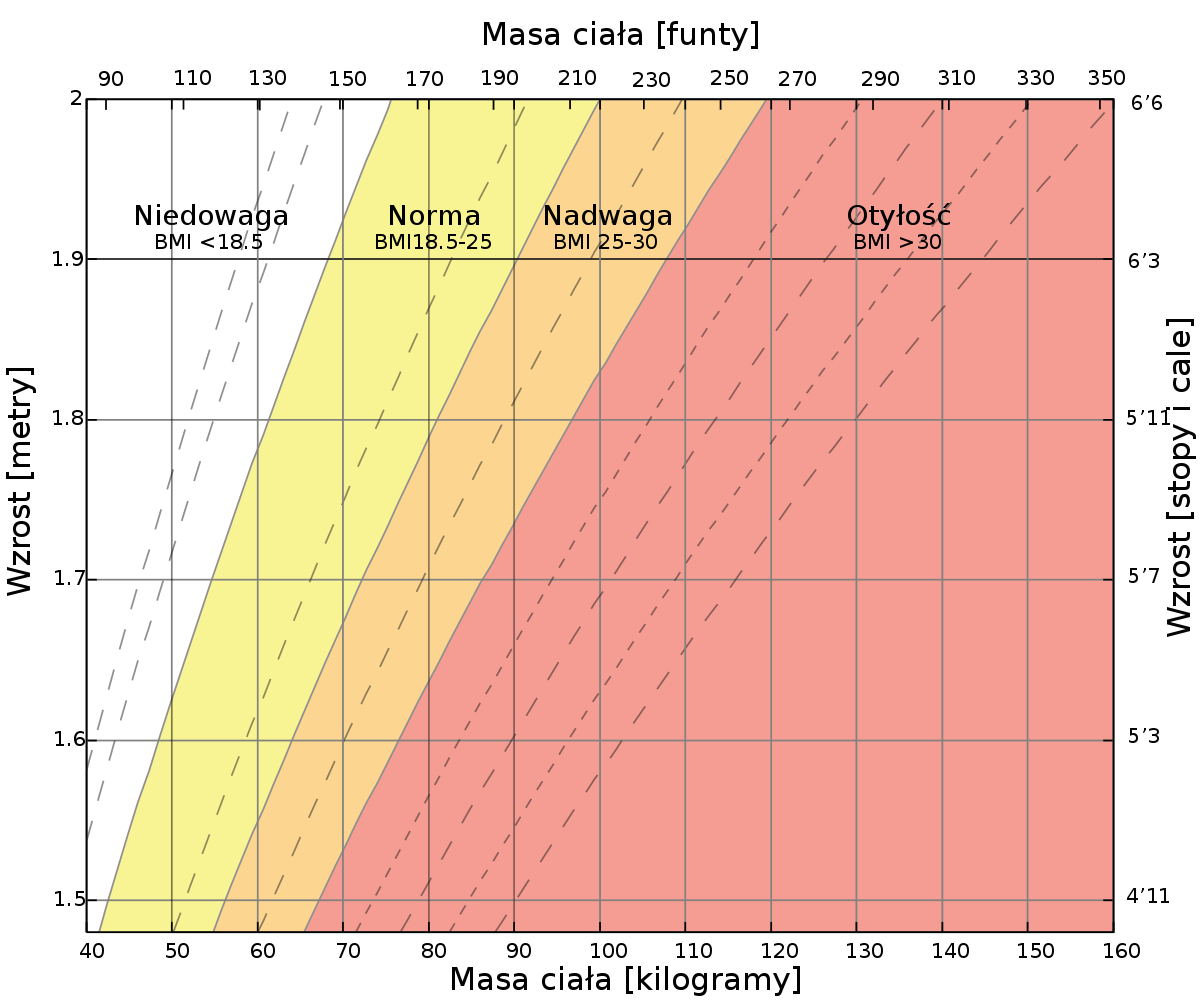
\includegraphics[width=1\linewidth]{BMI}

\begin{Shaded}
\begin{Highlighting}[]
\NormalTok{min\_BMI }\OtherTok{\textless{}{-}} \FunctionTok{min}\NormalTok{(cardio}\SpecialCharTok{$}\NormalTok{BMI)}
\NormalTok{max\_BMI }\OtherTok{\textless{}{-}} \FunctionTok{max}\NormalTok{(cardio}\SpecialCharTok{$}\NormalTok{BMI)}

\NormalTok{BMI\_groups }\OtherTok{\textless{}{-}} \FunctionTok{cut}\NormalTok{(cardio}\SpecialCharTok{$}\NormalTok{BMI,}
                  \AttributeTok{breaks =} \FunctionTok{c}\NormalTok{(min\_BMI, }\FloatTok{18.5}\NormalTok{, }\DecValTok{25}\NormalTok{, }\DecValTok{30}\NormalTok{, max\_BMI),}
                  \AttributeTok{labels =} \FunctionTok{c}\NormalTok{(}\StringTok{"Niedowaga"}\NormalTok{, }\StringTok{"Norma"}\NormalTok{, }\StringTok{"Nadwaga"}\NormalTok{, }\StringTok{"Otyłość"}\NormalTok{)}
\NormalTok{)}
\CommentTok{\# BMI\_groups \textless{}{-} droplevels(BMI\_groups)}
\CommentTok{\#cardio$BMI \textless{}{-} BMI\_groups}
\CommentTok{\#cardio$BMI \textless{}{-} as.factor(cardio$BMI)}

\FunctionTok{head}\NormalTok{(BMI\_groups)}
\end{Highlighting}
\end{Shaded}

\begin{verbatim}
## [1] Niedowaga Norma     Nadwaga   Norma     Norma     Nadwaga  
## Levels: Niedowaga Norma Nadwaga Otyłość
\end{verbatim}

\section{Usuwanie nieużywanych poziomów oraz podmiana i
konwersja}\label{usuwanie-nieuux17cywanych-poziomuxf3w-oraz-podmiana-i-konwersja}

By uniknąć błędów usuwam niepotrzebnie utowrzone levele. Podmieniam
wartości podane w tabeli na utworzone zakresy. KOnwertuje na typ factor.

\begin{Shaded}
\begin{Highlighting}[]
\NormalTok{BMI\_groups }\OtherTok{\textless{}{-}} \FunctionTok{droplevels}\NormalTok{(BMI\_groups)}
\CommentTok{\#Smoking\_groups \textless{}{-} droplevels(Smoking\_groups)}
\CommentTok{\#AlcoholDrinking\_groups \textless{}{-} droplevels(AlcoholDrinking\_groups)}
\CommentTok{\#Stroke\_groups \textless{}{-} droplevels(Stroke\_groups)}
\CommentTok{\#AgeCategory\_groups \textless{}{-} droplevels(AgeCategory\_groups)}
\CommentTok{\#Diabetic\_groups \textless{}{-} droplevels(Diabetic\_groups)}
\CommentTok{\#PhysicalActivity\_groups \textless{}{-} droplevels(PhysicalActivity\_groups)}


\FunctionTok{head}\NormalTok{(BMI\_groups)}
\end{Highlighting}
\end{Shaded}

\begin{verbatim}
## [1] Niedowaga Norma     Nadwaga   Norma     Norma     Nadwaga  
## Levels: Niedowaga Norma Nadwaga Otyłość
\end{verbatim}

\section{Dane po przerobieniu}\label{dane-po-przerobieniu}

\begin{Shaded}
\begin{Highlighting}[]
\FunctionTok{head}\NormalTok{(cardio)}
\end{Highlighting}
\end{Shaded}

\begin{verbatim}
##   HeartDisease   BMI Smoking AlcoholDrinking Stroke AgeCategory Diabetic
## 1           No 16.60     Yes              No     No       55-59      Yes
## 2           No 20.34      No              No    Yes 80 or older       No
## 3           No 26.58     Yes              No     No       65-69      Yes
## 4           No 24.21      No              No     No       75-79       No
## 5           No 23.71      No              No     No       40-44       No
## 6          Yes 28.87     Yes              No     No       75-79       No
##   PhysicalActivity
## 1              Yes
## 2              Yes
## 3              Yes
## 4               No
## 5              Yes
## 6               No
\end{verbatim}

\section{Sieci}\label{sieci}

\begin{Shaded}
\begin{Highlighting}[]
 \CommentTok{\#if (!requireNamespace("BiocManager", quietly = TRUE))}
 \CommentTok{\#  install.packages("BiocManager")}
\CommentTok{\# BiocManager::install(c("graph", "RBGL", "Rgraphviz"))}
\CommentTok{\# a}
\end{Highlighting}
\end{Shaded}

\begin{Shaded}
\begin{Highlighting}[]
\CommentTok{\#siec\_hc \textless{}{-} hc(cardio)}
\end{Highlighting}
\end{Shaded}


\end{document}
